\begin{document}

\newcommand{\TODO}[1]{\todo[inline,color=red!20]{#1}}

\title{Cloudmesh in support of the\\NIST Big Data Architecture Framework}


\numberofauthors{2} 
\author{
\alignauthor
Gregor von Laszewski, Badi Abduhl-Wahid, Fugang Wang, Hyungro Lee, Geoffrey C. Fox\\
       \affaddr{Indiana University}\\
       \affaddr{Bloomington, IN}\\
       \email{laszewski@gmail.com}
\alignauthor
Wo Chang\\
       \affaddr{NIST Big Data Public Working Group}\\
       \affaddr{National Institute of Standards and Technology}\\
       \email{wo.chang@nist.gov}
}
\date{20 April 2013}

\maketitle

\listoftodos[Notes]

\begin{abstract}
  The National Institute of Standards (NIST) has provided a big data
  reference architecture and is currently attempting to validate that
  architecture. As part of our current efforts we have developed
  cloudmesh client a tool that sets its goal towards easily managing
  clouds, container, batch queues and bare metal infrastructure. It
  also allows the integration of defined software stacks that can be
  used to deploy complex and state-of-the-art frameworks with devOps
  tools. Cloudmesh is on purpose designed to be vendor agnostic. We
  evaluate in this paper two aspects. First, based on our rich
  experience with clouds and other infrastructures, {\it can we verify the
  NIST reference architecture from our point of view?} Second, {\it which
  limitations may exist in cloudmesh client that need to be addressed
  to potentially improve integration with the NIST efforts?}  We will
  see in this paper that cloudmesh validates the NIST big data
  architecture which itself motivated further improvements to
  cloudmesh that we have implemented.
\end{abstract}


\section{Introduction}

In this section we provide some background information to motivate our
work and to introduce the two frameworks motivating this paper. This
includes cloudmesh \cite{las12-cloud} \cite{github-cloudmesh-client}
and the NIST big data reference architecture \cite{nist-bd}.

We start by giving brief introductions to the National Institute of
Standards (NIST) big data reference architecture (Section \ref{S:NBDarch}) followed
by a brief introduction to Cloudmesh (Section \ref{S:cmclient}).


We then \TODO{describe the next sections} 

\section{NBD Reference Architecture}
\label{S:NBDarch}

Commercial, academic, and government leaders agree about the potential
of {\em} Big Data to spark innovation, fuel commerce, and drive
progress. Big Data is the common term used to describe the deluge of
data in today’s networked, digitized, sensor-laden, and information
driven world \cite{nist-bd}. Desirable is as a vendor neutral,
technology- and infrastructure-agnostic conceptual model and examine
related issues.  The NIST big data working group is exploring pathways
forward in this direction which can be leveraged by the community. The
current result reference architecture is summarized in
\cite{nist-bd}. From this document we gather that the {\it
  ``conceptual model, referred to as the NIST Big Data Reference
  Architecture (NBDRA), was crafted by examining publicly available
  Big Data architectures representing various approaches and
  products. Inputs from the other NBD-PWG subgroups were also
  incorporated into the creation of the NBDRA. It is applicable to a
  variety of business environments, including tightly integrated
  enterprise systems, as well as loosely coupled vertical industries
  that rely on cooperation among independent stakeholders. The NBDRA
  captures the two known Big Data economic value chains: information,
  where value is created by data collection, integration, analysis,
  and applying the results to data-driven services, and the
  information technology (IT), where value is created by providing
  networking, infrastructure, platforms, and tools in support of
  vertical data-based applications.''}  It will produce a number of
documents related to definitions \cite{??}, taxonomies \cite{??}, use
cases and general requirements \cite{??}, security and privacy
\cite{??}, architectures white paper survey \cite{??}, reference
architecture \cite{??}, standards roadmap \cite{??}, and an interface
definition \cite{??}.

\TODO{Hyungro: add citations to the NIST documents related to this}

One of the desired tasks is to identify existing frameworks and to
analyze how they correlate to the current reference architecture
\cite{nist-bd}. This is conducted in order to validate and if needed
to improve the architecture.  The current NIST big data reference
architecture is shown in Figure~\ref{F:NIST-arch}. However we have
augmented the architecture with areas where cloudmesh interfaces with
it. We will describe the offerings in relationship to this
architecture of cloudmesh in detail in Section \ref{S:cm-nist}.  The
NIST BDA contains according to \cite{nist-bd} the following
components and services:

\TODO{find uniform abbreviation}

\TODO{define a cm nist section}

\begin{figure}[hp]
  \centering
     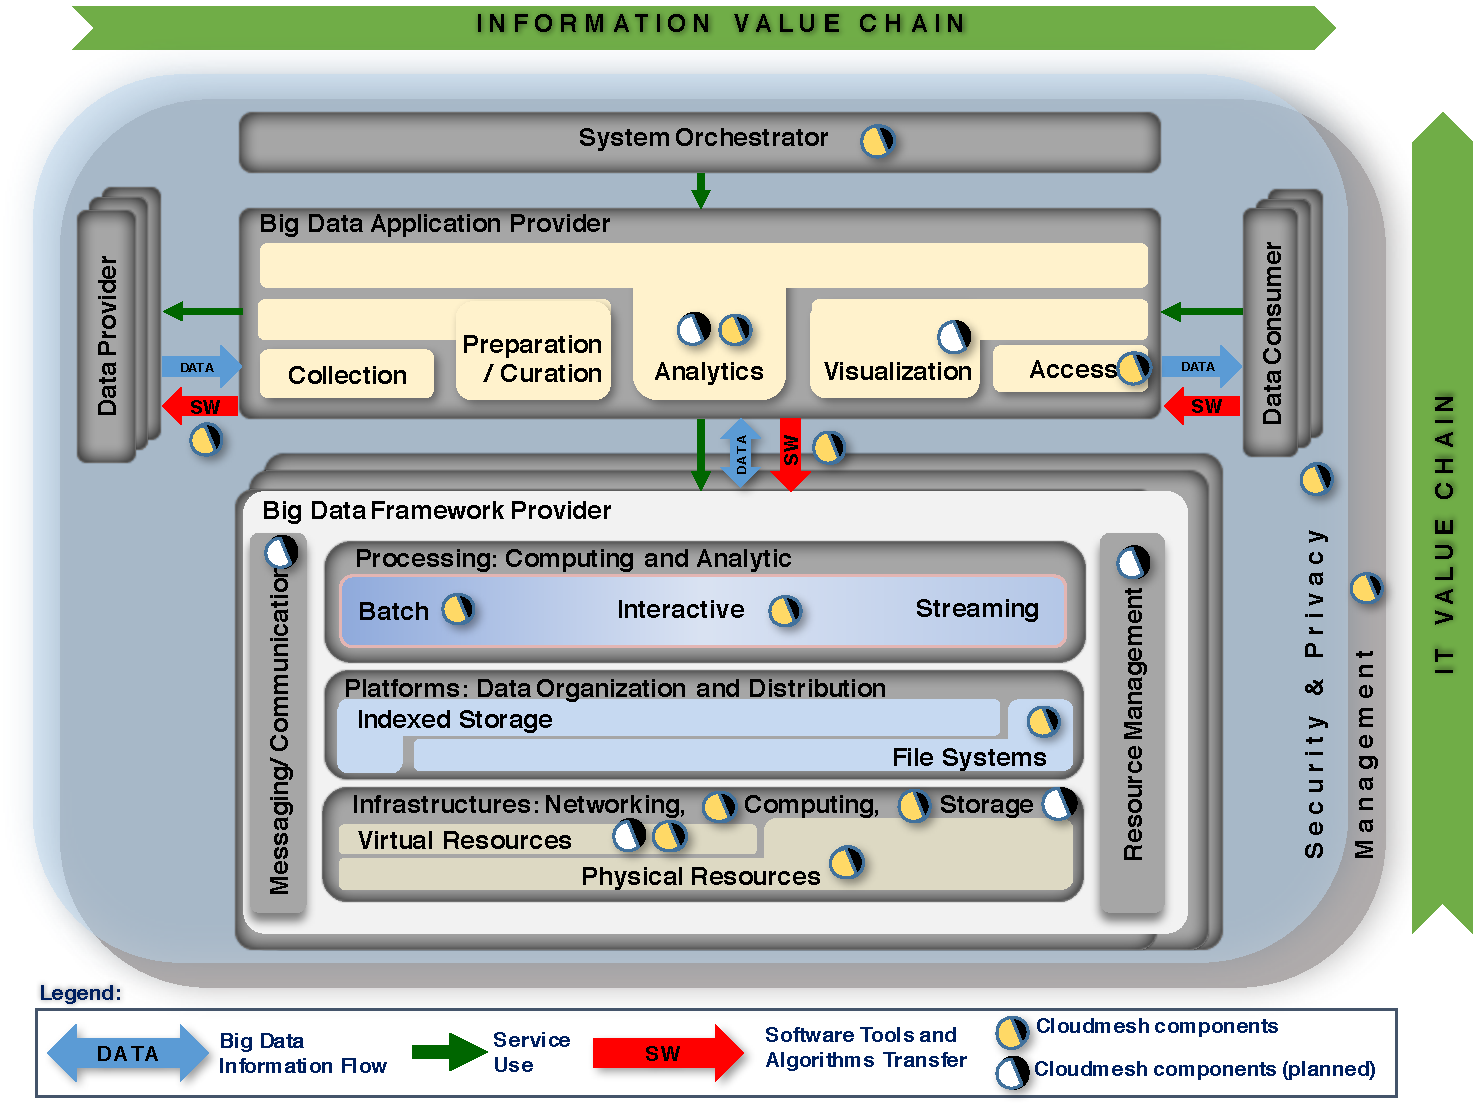
\includegraphics[width=1.0\columnwidth]{images/nist-bda.pdf}
  \caption{NIST Big Data Reference Architecture (NBDRA) diagram} 
  \label{F:NIST-arch}
%\end{figure}

\bigskip
%\begin{figure}[htb]
  \centering
     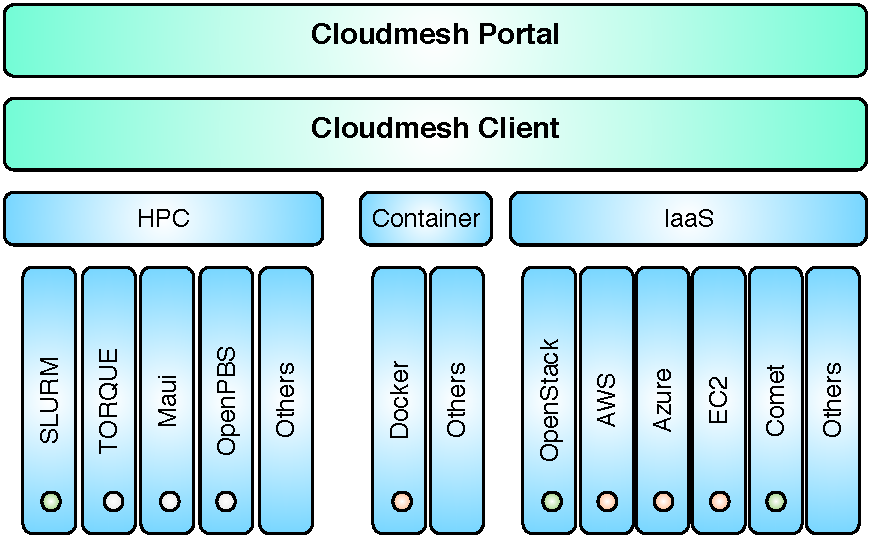
\includegraphics[width=1.0\columnwidth]{images/cloudmesh-arch-1.pdf}
  \caption{Cloudmesh layered architecture.} 
  \label{F:NIST-arch}
%\end{figure}
\bigskip

%\begin{figure}[htb]
  \centering
      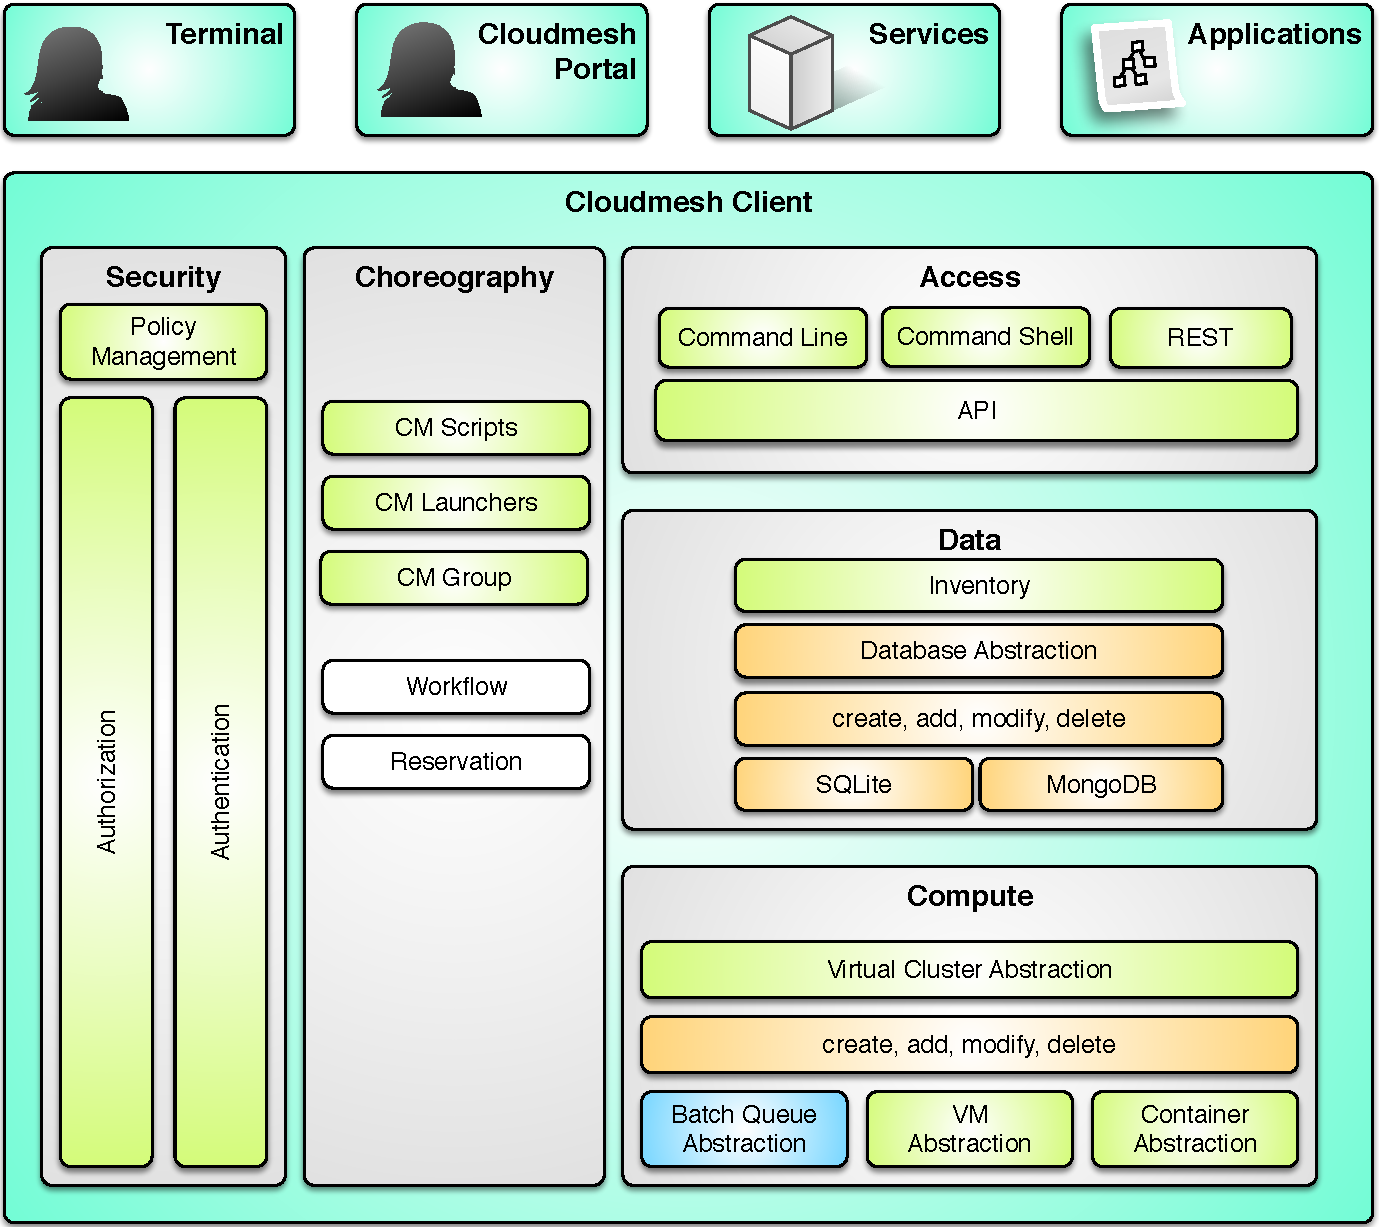
\includegraphics[width=1.0\columnwidth]{images/cloudmesh-arch-2.pdf}
  \caption{Cloudmesh components.} 
  \label{F:NIST-arch}
\end{figure}

\begin{figure}[hp]
  \centering
      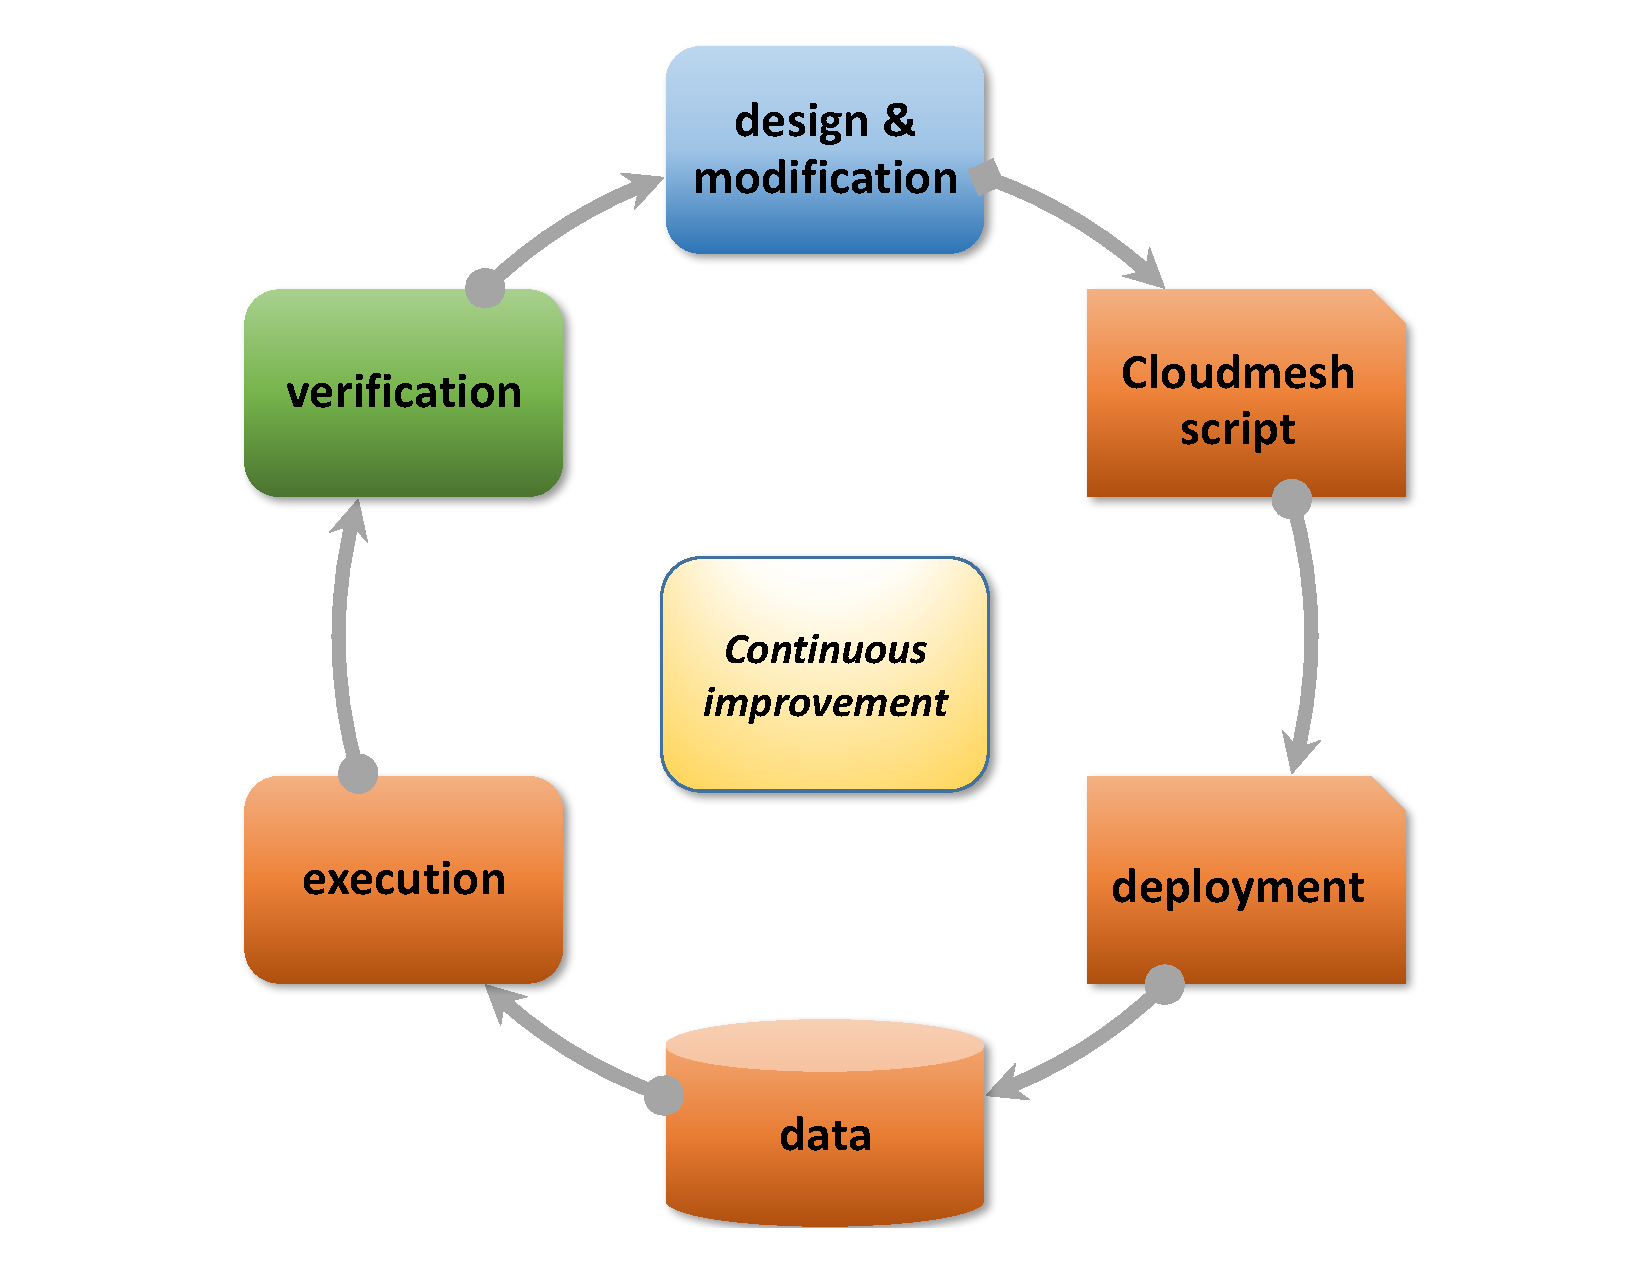
\includegraphics[width=1.0\columnwidth]{images/nist-devops-1.pdf}
  \caption{Continuous improvement while using cloudmesh interactively.}
  \label{F:NIST-arch}
%\end{figure}

\bigskip

%\begin{figure}[htb]
  \centering
      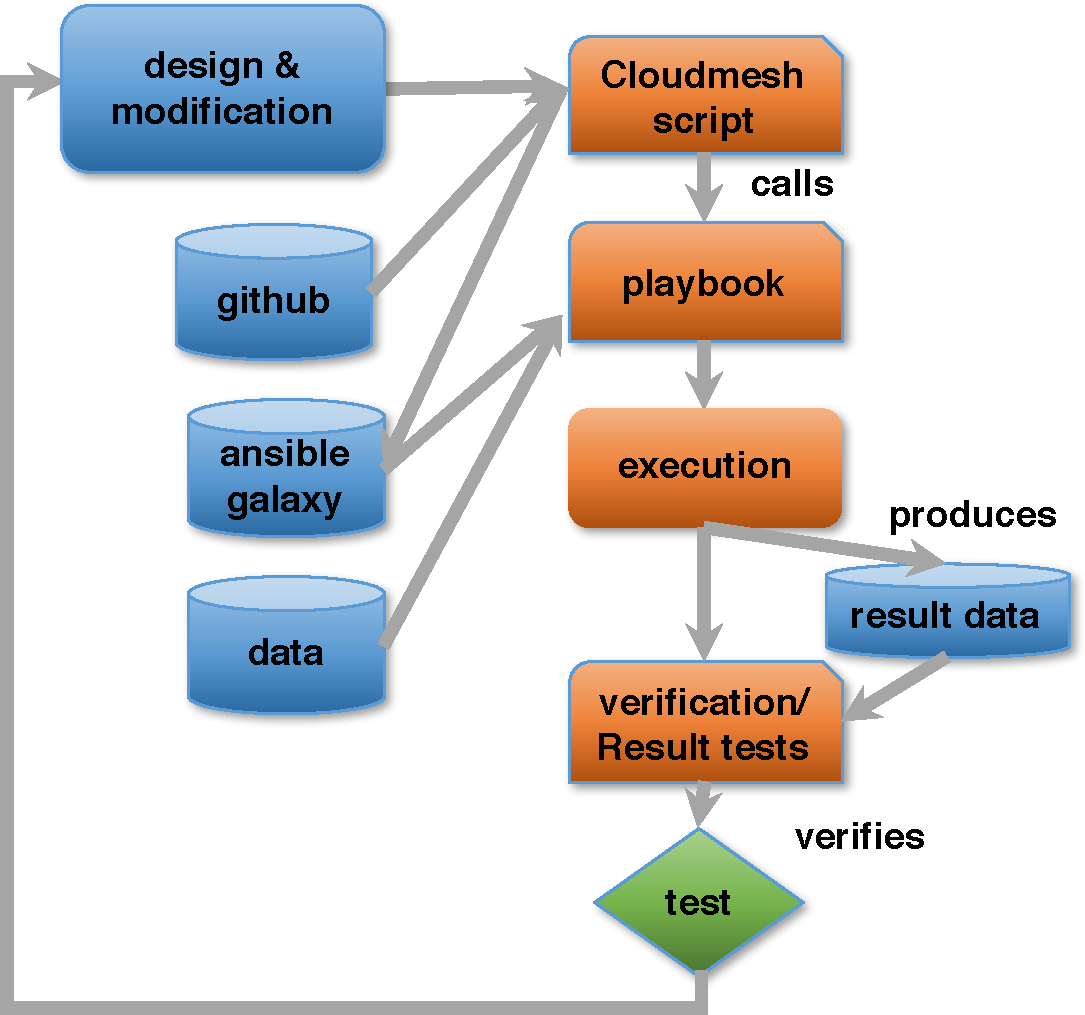
\includegraphics[width=0.8\columnwidth]{images/nist-devops-2.pdf}
  \caption{Interaction of the continuous improvement steps with
    various databases while using ansible deployment scripts.}
  \label{F:NIST-arch}
\end{figure}




\begin{description}

\item {\bf System Orchestrator} - provides high-level design dataflow
  between analytics tools and given datasets, computing system
  requirements, monitoring system resource and performance. At times
  the system orchestration is performed by the data scientist in an
  interactive manner. The system orchestrator is a service or
  component that acts in behalf of the data scientist, or another data
  science service that would require a particular configuration.

\item {\bf Data Provider} - provides abstraction of various types of 
data sources (such as raw data or data previously transformed by another system) 
and makes them available through different functional interfaces. This includes 
transfer analytics codes to data sources for effective analytic processing.


\item {\bf Big Data Application Provider} - provides analytics processing 
throughout the data lifecycle - acquisition, curation, analysis, visualization, 
and access - to meet requirements established by the System Orchestrator.


\item {\bf Big Data Framework Provider} - provides one or more instances 
of computing environment to support general Big Data tools, distributed file systems, 
and computing infrastructure - to meet requirements established by the Big Data 
Application Provider.


\item  {\bf Data Consumer} - provides interface to receive the value output 
from this NBD-RA ecosystem.


\item  {\bf Security and Privacy Fabric} - provides System Orchestrator 
the security and privacy interaction to the rest of the NBD-RA components to ensure 
protection of data and their content.


\item {\bf Management Fabric} - provides System Orchestrator the management 
interaction to the rest of the NBD-RA components with versatile system and software 
provisioning, resource and performance monitoring, while maintaining a high level 
of data quality and secure accessibility.

\end{description}


The focus of this document is on the Big Data Application Provider for how Big 
Data analytics can be applied/performed at each of its subcomponents. For the given 
mass amount of complex data, the process may involve one or more machine learning 
or analytic processing techniques at each of the subcomponents. 



\section{Cloudmesh Client}
\label{S:cmclient}

The cloudmesh client toolkit is a lightweight client interface of
accessing heterogeneous clouds, clusters, and workstations right from
the users computer. The user can manage his own set of resources he
would like to utilize. Thus the user has the freedom to customize
their cyber infrastructure they use. Cloudmesh client includes an API,
a commandline client, and a commandline shell. It strives to abstract
backends to databases that are used to manage the workflow utilizing
the different infrastructure and also the services. Switching for
example to stage virtual machines from openstack clouds to amazon is
as simple as specifying the name of the cloud. Moreover, cloudmesh
client can be installed on Linux, MacOSX, and even Windows. Currently
we support backends to SLURM, SSH, Openstack, Heat. In the past we
supported AWS and Azure. We are in the process of integrating them
back into the client.


Cloudmesh client allows to easily manage virtual machines, containers,
HPC tasks, through a convenient client and API. Hence cloudmesh is not
only a multi-cloud, but a multi-hpc environment that allows also to
use container technologies (under development).

\begin{description}

\item{\bf Client based.} Cloudmesh client as the name indicates is a
client based toolkit that is installed and run on the users
computers. This also includes an add on component to the cloudmesh
client which is a portal. Hence we distinguish the client that
contains most of the functionality, as well as a portal that can
access the functionality through a locally maintaine Web
portal. Important to note is that the user manages its own credentials
and thus security and credential management is done directly on the
users machine instead through a hosted Web portal. This increases the
security as access to any credential is managed by the user and is not
part of a credential management system.

\item{\bf Layered Architecture.} Cloudmesh client has a layered
architecture that allows easy development of new features. This also
allows contribution by the community while developing integrated and
smaller sub components. Figure A depicts the various layers. A
resource abstraction layer allows the integration of a multitude of
resources spanning HPC, Containers, and Cloud resources. (At this time
we focus on Openstack and Slurm resources. We are working on
reintegrating resources such as Azure, AWS, Maui, Moab, and others
which we previously supported, as well as new resources such as
docker).

\item{\bf Management Framework.} Cloudmesh client contains a
management framework, and its components are depicted in Figure
B. cloudmesh allows easy management of virtual machines, containers,
and the data associated with them. We are currently developing a
choreography framework that leverages Ansible, chef, and heat. All of
the functionality is easily usable through a command shell that also
can be used from the command line, and a Python API. IN future we will
be providing a REST API.

\item{\bf Database Agnostic.} Cloudmesh contains some state about the
resource and environment that a user may want to use. The information
is managed in an database abstraction that would allow storing the
data in a variety of databases such as SQL and MongoDB. At this time
we have chosen SQLite to be the default database as it does not
require any additional setup and is universally available on all
operating systems without change.

\item{\bf Command shell and line.} Cloudmesh contains a command shell
allowing scripts to be developed and run. However we designed the
command shell in such a way that each command can also be called from
the command line. Through the cloudmesh state machine the state
between command shell, command client, and the portal is shared.

\item{\bf Cloudmesh Client Portal.} Previously, we distributed
cloudmesh with client, server, and a portal components in one
package. This however turned out to be to complex to be installed for
some of our less technically skilled user community. Thus we split up
the install into two independent packages. The cloudmesh client and
the cloudmesh portal. The portal provides some elementary features to
manage virtual machines and HPC jobs. At this time the portal is
considered to be alpha technology. Just as the client the portal is to
be run on the local user machine in oredr to allow increased security
by managing the credentials locally rather than on a server.

\item{\bf Cloudmesh Two Factor Authentication.} We have an
exploratory project in place that looks at the use of Yubikeys for
cloudmesh, client and cloudmesh portal.

\item{\bf Cloudmesh Comet.} We are actively developing the client
interface for SDSC’s comet supercomputer allowing bare metal
provisioning. The interface reuses cloudmesh components and
technologies while interfacing with the comet cloud REST
interface. The goal here is to manage virtual clusters.

\end{description}

\section{DESIGN}



\subsection{Goals}


<Goals statement> 

technology agnostic
easy to use
expandable
comprehensive


\subsection{Approach}



<Approach description>


\section{Selected Cloudmesh Components}

\subsection{cm hpc run SCRIPT}

submits the script to the cluster. The script will be copied prior to
execution into the home directory on the remote machine. If a DIR is
specified it will be copied into that dir.  The name of the script is
either specified in the script itself, or if not the default naming
scheme of cloudmesh is used using the same index incremented name as
in vms fro clouds: cloudmes husername-index



\begin{table*}[htb]
\caption{Selected Service Description}
\begin{center}
\begin{tabular}{|p{8cm}|p{9cm}|}
\hline
\blue \textbf{URL} & \blue \textbf{Description}\tabularnewline
\hline
\multicolumn{2}{|l|}{\grey\bf Virtual Cluster} \tabularnewline
\hline
cluster/list & TBD \tabularnewline
\hline
cluster/delete?id=<id> & TBD \tabularnewline
\hline
cluster/status?id=<id> & TBD \tabularnewline
\hline
cluster/create?provider=<provider> & TBD \tabularnewline
\hline
\multicolumn{2}{|l|}{\grey\bf Stack} \tabularnewline
\hline
stack/delete?id=<id> & TBD \tabularnewline
\hline
stack/status?id=<id> & TBD \tabularnewline
\hline
stack/create?cluster=<cluster> & TBD \tabularnewline

\hline
\multicolumn{2}{|l|}{\grey\bf Batch Experiments} \tabularnewline
\hline
hpc/run?script=<scriptname>\&cluster=<clustername>& submits an experiment to the named
                               cluster and returns the unique hpc
                               experiment id\tabularnewline
\hline
hpc/status?id=<id> & returns the status of the job started with the run
                  command \tabularnewline
\hline
hpc/delete?id=<id> & deletes the experiment with the given id\tabularnewline
\hline
 hpc/list & list all jobs started with the run command \tabularnewline
\hline
\end{tabular}
\end{center}
\end{table*}


\subsection{Implementation}

When developing solutions and examples for this book, I used the software and programming 
environments listed in Table~P-3.

\begin{table}[htb]
\caption{Software/programming environments}
\begin{center}
\begin{tabular}{|l|l|}
\hline
\textbf{Software} & \textbf{Version}\tabularnewline
\hline
Python &2.7.12\tabularnewline
\hline
Ansible & 2.3 \tabularnewline
\hline
Operating system& Linux, OSX, (Windows)\tabularnewline
\hline
Cloudmesh client &  4.3.7 \tabularnewline
\hline
\end{tabular}
\end{center}
\end{table}

All programs in this book were tested with Java/JDK7, Hadoop 2.5.0, and Spark (1.1.0, 
1.3.0, 1.4.0). Examples are given in mixed operating system environments (Linux 
and OS X). For all examples and solutions, I engaged basic text editors (such as 
vi, vim, and TextWrangler) and compiled them using the Java command-line compiler 
(javac).


In this book, shell scripts (such as bash scripts) are used to run sample MapReduce/Hadoop 
and Spark programs. Lines that begin with a \$ or \# character indicate that the 
commands must be entered at a terminal prompt (such as bash).

\section{Stack}


Big Data Stack
Introduction
The Big Data Stack (BDS) tackles the problem of reproducibly deploying a stack of software packages that need to be coordinated for analyzing Big Data. Given a cluster of machines, BDS deploys and configures a user-defined subset of the available modules. A number of modules are available (e.g. Apache Spark, Apache Drill) that the user can use to customize the cluster environment. The ultimate goal is to minimize the amount of work and complexity required to obtain a functional stack for big data analytics.

BDS was initially developed to aid students in completing data analytics projects. Consistently students would want to use various technologies and would get stuck during the installation and configuration phase, unable to progress. Since this inception, BDS has been adapted to be used in other scenarios, such as developing use cases for the study of Big Data projects.

BDS is available online at https://github.com/futuresystems/big-data-stack
Terms and Definitions
Big Data: data sets too large to fit on a single machine or whose analysis is infeasible on a single machine, required a large cluster of networked computers.
BDS: Big Data Stack
Role: an Ansible Role
Playbook: an Ansible Playbook
Module: a standalone deployment of a service for BDS defined as a playbook
Usage
Requirements: Git, Python 2.7, Ansible, SSH, IP addresses of the cluster machines

Assumptions for below:
The repository has been cloned and the current working directory is located inside the local copy
The IP addresses are accessible via ssh
The cluster is running Ubuntu 14.04 and as a user ubuntu with sudo privileges
The IP addresses are given in the shell variables $IP1, $IP2, $IP3, and $IP4

The first step is to define the cluster. This step assigns labels that will be used during deployment and configuration to subsets of the machines in the cluster

\begin{Verbatim}[fontfamily=helvetica]
$ ./mk-inventory -n mycluster $IP1 $IP2 $IP3 $IP4 \
                            > inventory.txt
\end{Verbatim}

The second step is to deploy Hadoop as this a requirement for installing the modules:

\begin{Verbatim}[fontfamily=helvetica]
$ ansibile-playbook play-hadoop.yml
\end{Verbatim}

Next, a subset of the modules (found in the addons directory) can be deployed:

\begin{Verbatim}[fontfamily=helvetica]
$ ansible-playbook addons/spark.yml addons/hive.yml \
                               addons/drill.yml
\end{Verbatim}

At this point Hadoop, Apache Spark, Apache Hive, and Apache Drill will have been installed and configured for use. The user may now log into the cluster and begin useing these tools.


\subsection{Use Case: Fingerprint Matching}

\subsection{Deployment Tools}
This section describes various deployment tools and approaches

\paragraph{SSH+Scripts}
\paragraph{Ansible}
\paragraph{Chef}
\paragraph{Puppet}
\paragraph{Salt}

\subsection{Defining Modules}
A BDS module is a playbook 

\subsection{Defining Roles}

\begin{Verbatim}[fontfamily=helvetica]
stack check [--stack=bds]
stack init [--no-activate] [--branch=master] [--user=$USER] 
               [--name=<project>] <ip>...
stack list [--sort=<field=date>] [--list=<field,...=all>] [--json]
stack project [<name>]
stack deploy [<play>...] [--define=<define>...]

Options:
   --format=FORMAT  the output format [default: table]
   --cloud=CLOUD    the cloud name
\end{Verbatim}

\subsubsection{Example}

The following example assumes that a cluster (Ubuntu
14.04) has been launched already and can be accessed by
the 'ubuntu` user at addresses 10.0.0.10, 10.0.0.11, and
10.0.0.12.


\begin{Verbatim}[fontfamily=helvetica]
cm stack check
\end{Verbatim}
verify the environment


\begin{Verbatim}[fontfamily=helvetica]
cm stack init --user ubuntu 10.0.0.10 10.0.0.11 10.0.0.12
\end{Verbatim}

create a project for the cluster with given username and addresses


\begin{Verbatim}[fontfamily=helvetica]

\end{Verbatim}

\begin{Verbatim}[fontfamily=helvetica]

\end{Verbatim}

\begin{Verbatim}[fontfamily=helvetica]
cm stack project
\end{Verbatim}

get the name of the project

\begin{Verbatim}[fontfamily=helvetica]
cm stack deploy play-hadoop.yml addons/spark.yml addons/hbase.yml
\end{Verbatim}

deploy hadoop, spark, and hbase to the cluster

\section{Use Cases}


\section{51 NIST Benchmarking Examples for Big Data}

\begin{description}

\item[Government Operation:] National Archives and Records
  Administration, Census Bureau

\item[Commercial:] Finance in Cloud, Cloud Backup, Mendeley
  (Citations), Netflix, Web Search, Digital Materials, Cargo shipping
  (as in UPS)

\item[Defense:] Sensors, Image surveillance, Situation Assessment
  Healthcare

\item[Life Sciences:] Medical records, Graph and Probabilistic
  analysis, Pathology, Bioimaging, Genomics, Epidemiology, People
  Activity models, BiodiversityDeep Learning and Social Media: Driving
  Car, Geolocate images/cameras, Twitter, Crowd Sourcing, Network
  Science, NIST benchmark datasets

\item[The Ecosystem for Research:] Metadata, Collaboration, Language
  Translation, Light source experiments

\item[Astronomy and Physics:] Sky Surveys compared to simulation,
  Large Hadron Collider at CERN, Belle Accelerator II in JapanEarth,

\item[Environmental and Polar Science:] Radar Scattering in
  Atmosphere, Earthquake, Ocean, Earth Observation, Ice sheet Radar
  scattering, Earth radar mapping, Climate simulation datasets,
  Atmospheric turbulence identification, Subsurface Biogeochemistry
  (microbes to watersheds), AmeriFlux and FLUXNET gas sensors

\item[Energy:] Smart grid

\end{description}

\begin{table*}[htb]

\caption{table of usecases}
\label{T:usecases}

TABLE COME HERE

\end{table*}


\section{Conclusion}

<Description> 

\subsection{Lessons Learned}

<General description>

\subsection{Future Works}


<General description>

\documentclass{article}
\usepackage{csvsimple}
\usepackage{longtable}
\usepackage{lscape}
\usepackage{array,graphicx}
\usepackage{booktabs}
\usepackage{pifont}
\usepackage{geometry}

\newcommand*\rot{\rotatebox{90}}
\newcommand*\OK{\ding{51}}
\newcolumntype{L}{>{\centering\arraybackslash}m{4cm}}

\begin{filecontents*}{list_of_projects_with_roles.csv}
ID,Use Case,Source,Hadoop,Mesos,Spark,Storm,Pig,Hive,Drill,HDFS,HBase,Mysql,MongoDB,RethinkDB,Mahout,D3 and Tableau,nltk,MLlib,Lucene/Solr,OpenCV,Python,Java,maven,Ganglia,Nagios,spark supervisord,zookeeper,AlchemyAPI,R,dataset,dataset size (GB)
 U.N1,NIST Fingerprint Matching,NIST,*,,*,,,*,*,,*,*,,,,,,,,,,*,*,*,*,*,*,,,Special Database 14 - NIST Mated Fingerprint Card Pairs 2.,2.1
 U.N2,Human and Face Detection,NIST,,*,*,,,,,,,,,,,,,,,*,*,,, ,,,*,,,INRIA Person Dataset,0.96
 U.N3,Twitter Analysis,NIST,,,,*,,,,,*,,*,,,*,*,,,,*,*,,,,,*,*,*,Twitter,
 U.N4,Analytics for Healthcare Data/Health Informatics,NIST,*,,*,,,,,,*,,,,*,*,,*,*,,,*,, ,,,*,,,Medicare Part-B in 2014 from Center for Medicare and Medicaid Services (CMS),0.1
 U.N5,Spatial Big Data/Spatial Statistics/Geographic Information Systems,NIST,*,,*,,,,,,,,,,*,*,,*,,,,*,*,,,,,,,Uber,0.2
 U.N6,Data Warehousing and Data Mining,NIST,*,,*,,*,*,,,*,,*,,*,*,,*,*,,,*,,,,,*,,,,count,,,,4,1,5,1,1,2,1,0,4,1,2,0,3,4,1,3,2,1,2,5,2,3,1,1,5,1,1,,
 \end{filecontents*}

\begin{document}

\newgeometry{margin=1cm}
\begin{table} \centering
  \begin{tabular}{@{} cl*{26}c @{}}
    & ID & \rot{Hadoop} & \rot{Mesos} & \rot{Spark} & \rot{Storm} & \rot{Pig} & \rot{Hive} & \rot{Drill} & \rot{HDFS} & \rot{HBase} & \rot{Mysql} & \rot{MongoDB} & \rot{RethinkDB} & \rot{Mahout} & \rot{D3 and Tableau} & \rot{nltk} & \rot{MLlib} & \rot{Lucene/Solr} & \rot{OpenCV} & \rot{Python} & \rot{Java} & \rot{Ganglia} & \rot{Nagios} & \rot{zookeeper} & \rot{AlchemyAPI} & \rot{R} & \rot{\shortstack{dataset\\ size (GB)}} \\
    \hline
    & U.N1 & \OK &  & \OK &  &  & \OK & \OK &  & \OK & \OK &  &  &  &  &  &  &  &  &  & \OK & \OK & \OK & \OK &  &  & 2.1 \\
    \hline
    & U.N2 &  & \OK & \OK &  &  &  &  &  &  &  &  &  &  &  &  &  &  & \OK & \OK &  &   &  & \OK &  &  & 0.96 \\
    \hline
    & U.N3 &  &  &  & \OK &  &  &  &  & \OK &  & \OK &  &  & \OK & \OK &  &  &  & \OK & \OK &  &  & \OK & \OK & \OK \\
    \hline
    & U.N4 & \OK &  & \OK &  &  &  &  &  & \OK &  &  &  & \OK & \OK &  & \OK & \OK &  &  & \OK &   &  & \OK &  &  & 0.1 \\
    \hline
    & U.N5 & \OK &  & \OK &  &  &  &  &  &  &  &  &  & \OK & \OK &  & \OK &  &  &  & \OK &  &  &  &  &  & 0.2 \\
    \hline
    & U.N6 & \OK &  & \OK &  & \OK & \OK &  &  & \OK &  & \OK &  & \OK & \OK &  & \OK & \OK &  &  & \OK &  &  & \OK &  &   \\

  \end{tabular}
 \end{table}

 \begin{tabular}{l|l|l|L}%
   \bfseries ID& \bfseries Use Case & \bfseries Source & \bfseries Dataset% specify table head
   \csvreader[head to column names]{list_of_projects_with_roles.csv}{}% use head of csv as column names
   {\\\hline\ID &\csvcolii &\Source &\dataset}% specify your coloumns here
 \end{tabular}

 \restoregeometry
\end{document}


\TODO{server less computing \cite{jil16}} 

\TODO{server less computing \cite{cloud3}} 
